\documentclass[journal,12pt,twocolumn]{IEEEtran}

\usepackage{setspace}
\usepackage{gensymb}

\singlespacing


\usepackage[cmex10]{amsmath}

\usepackage{amsthm}

\usepackage{mathrsfs}
\usepackage{txfonts}
\usepackage{stfloats}
\usepackage{bm}
\usepackage{cite}
\usepackage{cases}
\usepackage{subfig}

\usepackage{longtable}
\usepackage{multirow}

\usepackage{enumitem}
\usepackage{mathtools}
\usepackage{steinmetz}
\usepackage{tikz}
\usepackage{circuitikz}
\usepackage{verbatim}
\usepackage{tfrupee}
\usepackage[breaklinks=true]{hyperref}
\usepackage{graphicx}
\usepackage{tkz-euclide}
\usepackage{float}

\usetikzlibrary{calc,math}
\usepackage{listings}
    \usepackage{color}                                            %%
    \usepackage{array}                                            %%
    \usepackage{longtable}                                        %%
    \usepackage{calc}                                             %%
    \usepackage{multirow}                                         %%
    \usepackage{hhline}                                           %%
    \usepackage{ifthen}                                           %%
    \usepackage{lscape}     
\usepackage{multicol}
\usepackage{chngcntr}

\DeclareMathOperator*{\Res}{Res}

\renewcommand\thesection{\arabic{section}}
\renewcommand\thesubsection{\thesection.\arabic{subsection}}
\renewcommand\thesubsubsection{\thesubsection.\arabic{subsubsection}}

\renewcommand\thesectiondis{\arabic{section}}
\renewcommand\thesubsectiondis{\thesectiondis.\arabic{subsection}}
\renewcommand\thesubsubsectiondis{\thesubsectiondis.\arabic{subsubsection}}


\hyphenation{op-tical net-works semi-conduc-tor}
\def\inputGnumericTable{}                                 %%

\lstset{
%language=C,
frame=single, 
breaklines=true,
columns=fullflexible
}
\begin{document}
\newtheorem{theorem}{Theorem}[section]
\newtheorem{problem}{Problem}
\newtheorem{proposition}{Proposition}[section]
\newtheorem{lemma}{Lemma}[section]
\newtheorem{corollary}[theorem]{Corollary}
\newtheorem{example}{Example}[section]
\newtheorem{definition}[problem]{Definition}

\newcommand{\BEQA}{\begin{eqnarray}}
\newcommand{\EEQA}{\end{eqnarray}}
\newcommand{\define}{\stackrel{\triangle}{=}}
\bibliographystyle{IEEEtran}
\providecommand{\mbf}{\mathbf}
\providecommand{\pr}[1]{\ensuremath{\Pr\left(#1\right)}}
\providecommand{\qfunc}[1]{\ensuremath{Q\left(#1\right)}}
\providecommand{\sbrak}[1]{\ensuremath{{}\left[#1\right]}}
\providecommand{\lsbrak}[1]{\ensuremath{{}\left[#1\right.}}
\providecommand{\rsbrak}[1]{\ensuremath{{}\left.#1\right]}}
\providecommand{\brak}[1]{\ensuremath{\left(#1\right)}}
\providecommand{\lbrak}[1]{\ensuremath{\left(#1\right.}}
\providecommand{\rbrak}[1]{\ensuremath{\left.#1\right)}}
\providecommand{\cbrak}[1]{\ensuremath{\left\{#1\right\}}}
\providecommand{\lcbrak}[1]{\ensuremath{\left\{#1\right.}}
\providecommand{\rcbrak}[1]{\ensuremath{\left.#1\right\}}}
\theoremstyle{remark}
\newtheorem{rem}{Remark}
\newcommand{\sgn}{\mathop{\mathrm{sgn}}}
\providecommand{\abs}[1]{\vert#1\vert}
\providecommand{\res}[1]{\Res\displaylimits_{#1}} 
\providecommand{\norm}[1]{\lVert#1\rVert}
%\providecommand{\norm}[1]{\lVert#1\rVert}
\providecommand{\mtx}[1]{\mathbf{#1}}
\providecommand{\mean}[1]{E[ #1 ]}
\providecommand{\fourier}{\overset{\mathcal{F}}{ \rightleftharpoons}}
%\providecommand{\hilbert}{\overset{\mathcal{H}}{ \rightleftharpoons}}
\providecommand{\system}{\overset{\mathcal{H}}{ \longleftrightarrow}}
	%\newcommand{\solution}[2]{\textbf{Solution:}{#1}}
\newcommand{\solution}{\noindent \textbf{Solution: }}
\newcommand{\cosec}{\,\text{cosec}\,}
\providecommand{\dec}[2]{\ensuremath{\overset{#1}{\underset{#2}{\gtrless}}}}
\newcommand{\myvec}[1]{\ensuremath{\begin{pmatrix}#1\end{pmatrix}}}
\newcommand{\mydet}[1]{\ensuremath{\begin{vmatrix}#1\end{vmatrix}}}
\numberwithin{equation}{subsection}
\makeatletter
\@addtoreset{figure}{problem}
\makeatother
\let\StandardTheFigure\thefigure
\let\vec\mathbf
\renewcommand{\thefigure}{\theproblem}
\def\putbox#1#2#3{\makebox[0in][l]{\makebox[#1][l]{}\raisebox{\baselineskip}[0in][0in]{\raisebox{#2}[0in][0in]{#3}}}}
     \def\rightbox#1{\makebox[0in][r]{#1}}
     \def\centbox#1{\makebox[0in]{#1}}
     \def\topbox#1{\raisebox{-\baselineskip}[0in][0in]{#1}}
     \def\midbox#1{\raisebox{-0.5\baselineskip}[0in][0in]{#1}}
\vspace{3cm}
\title{Quiz 2}
\author{Dishank Jain \\ AI20BTECH11011}
\maketitle
\newpage
\bigskip
\renewcommand{\thefigure}{\theenumi}
\renewcommand{\thetable}{\theenumi}
Download python codes from
%
\begin{lstlisting}
https://github.com/Dishank422/EE3900/blob/main/quiz2/codes
\end{lstlisting}
%
and latex-tikz codes from 
%
\begin{lstlisting}
https://github.com/Dishank422/EE3900/blob/main/quiz2/latex_code.tex
\end{lstlisting}
%
\section{Discrete Time Signal Processing 3.7(b,c)}
The input to a causal linear time-invariant system is
\begin{equation}
    x[n] = u[-n-1]+\brak{\dfrac{1}{2}}^nu[n]
\end{equation}
The z-transform of the output of this system is 
\begin{equation}
    Y(z) = \dfrac{-\frac{1}{2}z^{-1}}{\brak{1-\frac{1}{2}z^{-1}}\brak{1+z^{-1}}}
\end{equation}
\begin{enumerate}[label=(\alph*)]
\setcounter{enumi}{1}
    \item What is the region of convergence for Y(z)?
    \item Determine y[n].
\end{enumerate}

\section{Solution}
\begin{lemma}
The Z-transform of the sequence $a^nu(n)$ is $\dfrac{1}{1-az^{-1}}$ with a region of convergence $\abs{z} > \abs{a}$.
\label{l1}
\end{lemma}
\begin{proof}
\begin{equation}
    \mathcal{Z}(a^nu(n)) = \sum_{n=0}^{\infty}a^nz^{-n} = \dfrac{1}{1-az^{-1}}
\end{equation}
ROC is given by $\abs{\dfrac{a}{z}} < 1$, i.e. $\abs{z} > \abs{a}$.
\end{proof}

\begin{lemma}
The Z-transform of the sequence $u(-n-1)$ is $\dfrac{-1}{1-z^{-1}}$ with a region of convergence $\abs{z} < 1$.
\label{l2}
\end{lemma}
\begin{proof}
\begin{equation}
    \mathcal{Z}(u(-n-1)) = \sum_{n=-\infty}^{-1}z^{-n} = \sum_{n=1}^{\infty}z^{n} = \dfrac{-1}{1-z^{-1}}
\end{equation}
ROC is given by $\abs{z} < 1$.
\end{proof}

\begin{enumerate}[label=(\alph*)]
\setcounter{enumi}{1}
    \item Using lemmas \ref{l1} and \ref{l2}, 
\begin{align}
    X(z) &= \mathcal{Z}(x[n])\\
         &= \mathcal{Z}(u[-n-1]) + \mathcal{Z}\brak{\brak{\dfrac{1}{2}}^nu[n]}\\
         &= \dfrac{-1}{1-z^{-1}} + \dfrac{1}{1-\frac{1}{2}z^{-1}}\\
         &= \dfrac{-\frac{1}{2}z^{-1}}{\brak{1-\frac{1}{2}z^{-1}}\brak{1-z^{-1}}}
\end{align}
The ROC of X(z) is the intersection $\abs{z} < 1$ and $\abs{z} > \frac{1}{2}$. Thus the ROC of X(z) is $\frac{1}{2} < \abs{z} < 1$. Since the system is causal, the ROC of H(z) is $\abs{z} > 1$. We also have
\begin{equation}
    H(z) = \dfrac{Y(z)}{X(z)}
\end{equation}

\begin{table}[h]
    \centering
    \begin{tabular}{|c|c|c|c|}
    \hline
         Region & $\frac{1}{X(z)}$ & H(z) & Y(z) \\
         \hline
         $\abs{z} < \frac{1}{2}$ & Converges & Doesn't & Must not \\
         & & converge & converge \\
         \hline
         $\frac{1}{2} < \abs{z} < 1$ & Converges & Doesn't & Must not \\
         & & converge & converge \\
         \hline
         $\abs{z} > 1$ & Converges & Converges & Must \\
         & & & converge \\
         \hline
    \end{tabular}
    \caption{ROC analysis for Y(z)}
    \label{analysis}
\end{table}
From table \ref{analysis}, it is clear that ROC of Y(z) is $\abs{z} > 1$.

Note that in $\frac{1}{2} < \abs{z} < 1$, $\frac{1}{X(z)}$ converges because the only zero of X(z) is $\abs{z} = 0$ which doesn't lie in this region.
\item 
\begin{align}
    Y(z) &= \dfrac{-\frac{1}{2}z^{-1}}{\brak{1-\frac{1}{2}z^{-1}}\brak{1+z^{-1}}}\\
         &= \dfrac{-\frac{1}{3}}{1-\frac{1}{2}z^{-1}} + \dfrac{\frac{1}{3}}{1+z^{-1}}
\end{align}
Using the fact that ROC of Y(z) is $\abs{z} > 1$ and using converse of lemma \ref{l1}, \begin{equation}
    y[n] = -\dfrac{1}{3}\brak{\dfrac{1}{3}}^nu[n] + \dfrac{
    1}{3}(-1)^nu[n]
\end{equation} 
\end{enumerate}

\begin{figure}[h]
    \centering
    \resizebox{\columnwidth}{!}{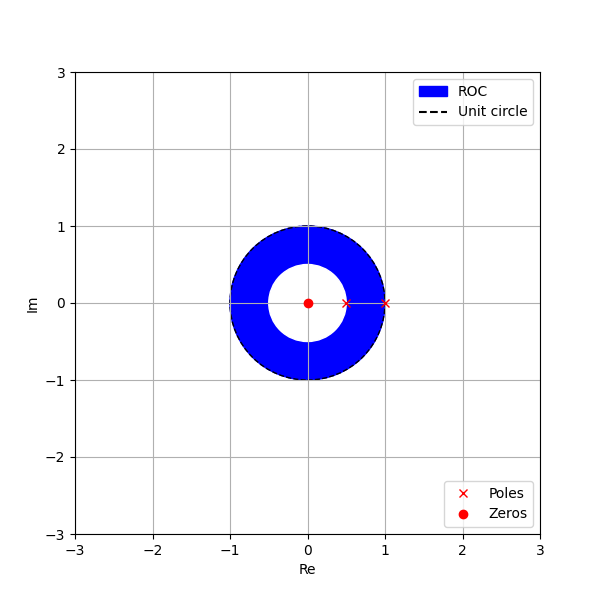
\includegraphics{figures/X(z).png}}
    \caption{ROC of X(z)}
\end{figure}

\begin{figure}[h]
    \centering
    \resizebox{\columnwidth}{!}{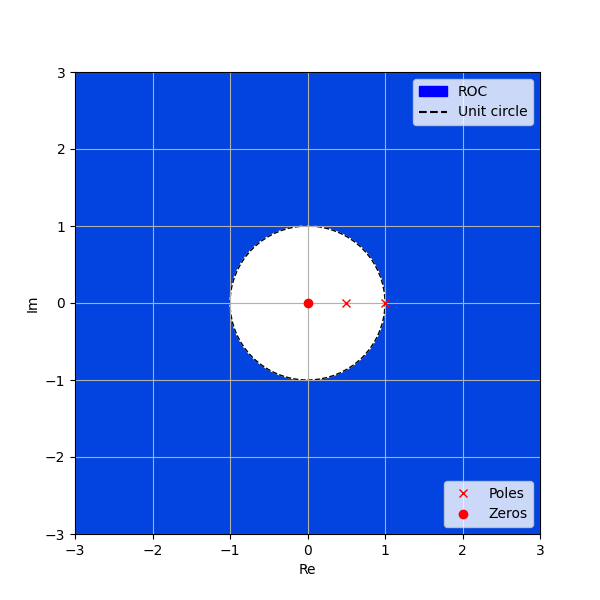
\includegraphics{figures/Y(z).png}}
    \caption{ROC of Y(z)}
\end{figure}

\begin{figure}[h]
    \centering
    \resizebox{\columnwidth}{!}{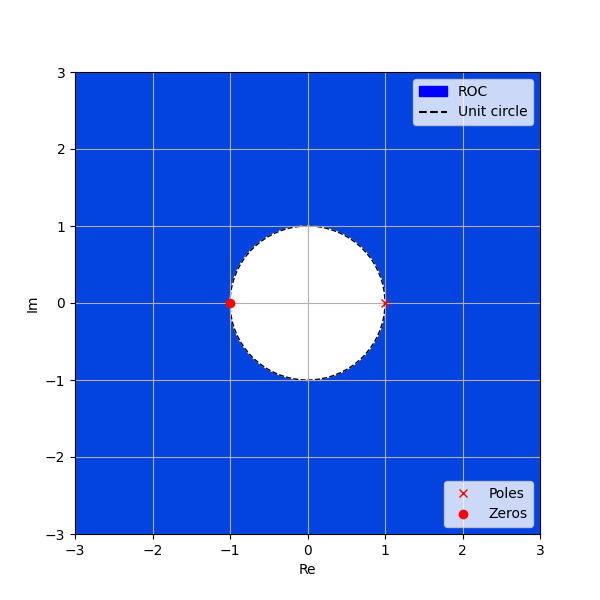
\includegraphics{figures/H(z).png}}
    \caption{ROC of H(z)}
\end{figure}

\begin{figure}[h]
    \centering
    \resizebox{\columnwidth}{!}{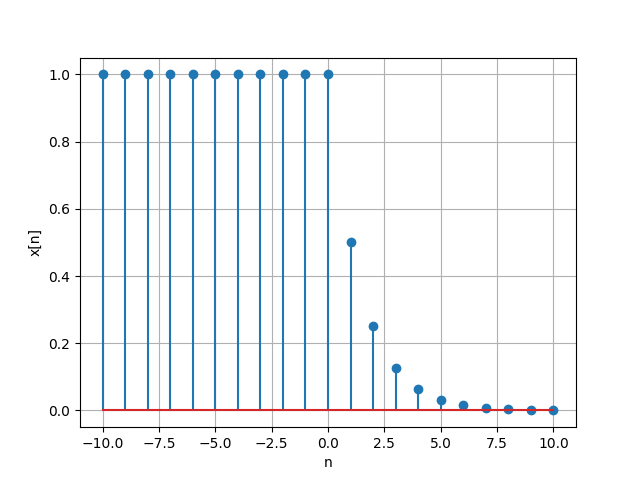
\includegraphics{figures/x[n].png}}
    \caption{x[n]}
\end{figure}

\begin{figure}[h]
    \centering
    \resizebox{\columnwidth}{!}{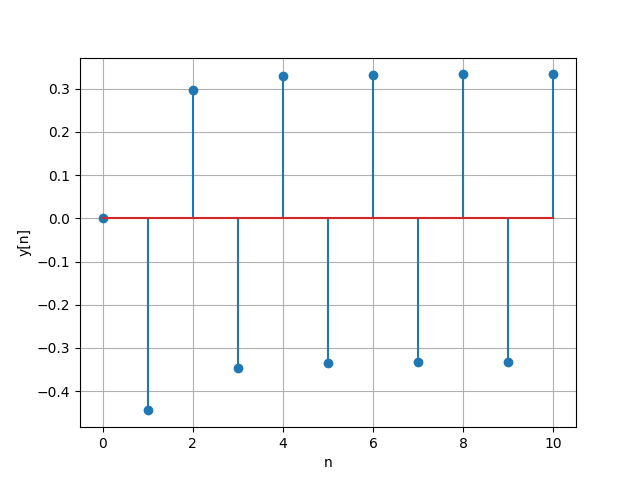
\includegraphics{figures/y[n].png}}
    \caption{y[n]}
\end{figure}
\end{document}
